\begin{minipage}{0.49\textwidth}
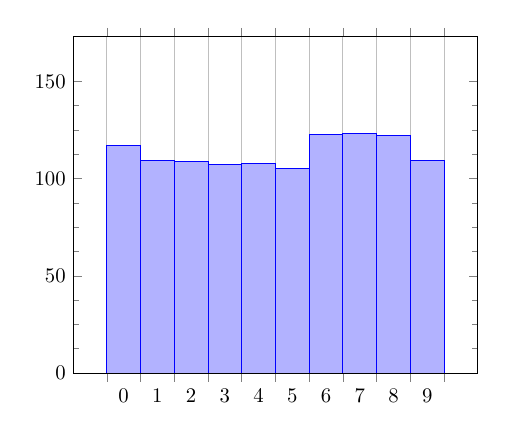
\begin{tikzpicture}[scale=0.75]
  \begin{axis}[ybar interval, ymax=172.943,ymin=0, minor y tick num = 3]
    \addplot coordinates { (0,116.844) (1,109.284) (2,108.984) (3,107.08) (4,107.645) (5,105.295) (6,122.603) (7,123.168) (8,122.029) (9,109.177) (10, 78.6104) };
  \end{axis}
\end{tikzpicture}
\caption*{Average weights repartitions on several trees}
\end{minipage}
\begin{minipage}{0.49\textwidth}
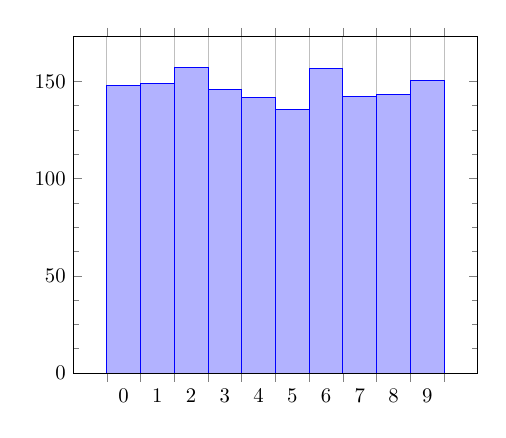
\begin{tikzpicture}[scale=0.75]
  \begin{axis}[ybar interval, ymax=172.943,ymin=0, minor y tick num = 3]
    \addplot coordinates { (0,147.98) (1,149.065) (2,157.221) (3,145.864) (4,141.521) (5,135.682) (6,156.605) (7,142.218) (8,143.256) (9,150.377) (10, 78.6104) };
  \end{axis}
\end{tikzpicture}
\caption*{Average weights repartitions on one of the trees}
\end{minipage}
\begin{minipage}{0.49\textwidth}
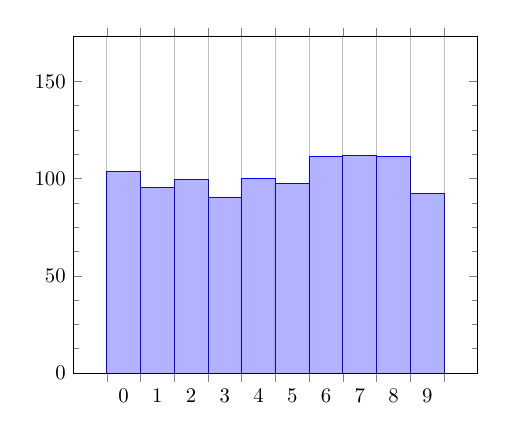
\begin{tikzpicture}[scale=0.75]
  \begin{axis}[ybar interval, ymax=172.943,ymin=0, minor y tick num = 3]
    \addplot coordinates { (0,103.839) (1,95.4839) (2,99.3821) (3,90.5136) (4,100.047) (5,97.5385) (6,111.633) (7,112.06) (8,111.325) (9,92.4615) (10, 78.6104) };
  \end{axis}
\end{tikzpicture}
\caption*{Average weights repartitions on one of the trees}
\end{minipage}
\begin{minipage}{0.49\textwidth}
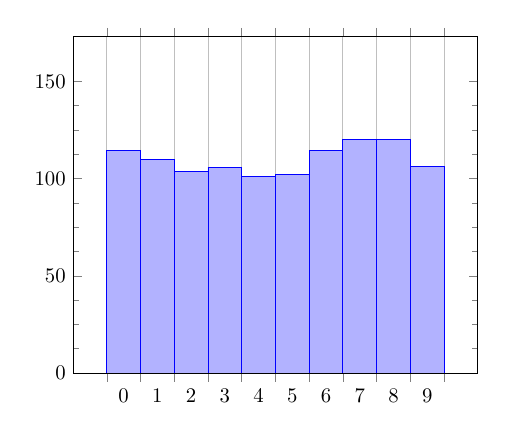
\begin{tikzpicture}[scale=0.75]
  \begin{axis}[ybar interval, ymax=172.943,ymin=0, minor y tick num = 3]
    \addplot coordinates { (0,114.583) (1,109.61) (2,103.548) (3,105.903) (4,101.238) (5,102.169) (6,114.268) (7,120.005) (8,120.007) (9,106.03) (10, 78.6104) };
  \end{axis}
\end{tikzpicture}
\caption*{Average weights repartitions on one of the trees}
\end{minipage}
